\documentclass[aspectratio=169,11pt]{beamer}

\usepackage[T1]{fontenc}
\usepackage{lmodern}
\usepackage{booktabs}
\usepackage{listings}
\usepackage{tikz}
\usetikzlibrary{arrows.meta,positioning,shapes.geometric}

% -----------------------------------------------------------------------------
% Visual design
% -----------------------------------------------------------------------------
\definecolor{Navy}{HTML}{172A3A}
\definecolor{Blue}{HTML}{0969DA}
\definecolor{LightBlue}{HTML}{EAF3FF}
\definecolor{Green}{HTML}{1A7F37}
\definecolor{LightGreen}{HTML}{EAF7ED}
\definecolor{Orange}{HTML}{BC4C00}
\definecolor{LightOrange}{HTML}{FFF1E5}
\definecolor{Red}{HTML}{CF222E}
\definecolor{LightRed}{HTML}{FFEBE9}
\definecolor{Ink}{HTML}{24292F}
\definecolor{Muted}{HTML}{57606A}
\definecolor{Rule}{HTML}{D0D7DE}
\definecolor{CodeBG}{HTML}{F6F8FA}

\setbeamercolor{normal text}{fg=Ink,bg=white}
\setbeamercolor{structure}{fg=Blue}
\setbeamercolor{frametitle}{fg=white,bg=Navy}
\setbeamercolor{title}{fg=white}
\setbeamercolor{subtitle}{fg=LightBlue}
\setbeamercolor{block title}{fg=white,bg=Blue}
\setbeamercolor{block body}{fg=Ink,bg=LightBlue}
\setbeamercolor{block title alerted}{fg=white,bg=Orange}
\setbeamercolor{block body alerted}{fg=Ink,bg=LightOrange}
\setbeamercolor{block title example}{fg=white,bg=Green}
\setbeamercolor{block body example}{fg=Ink,bg=LightGreen}

\setbeamertemplate{navigation symbols}{}
\setbeamertemplate{itemize item}{\color{Blue}$\blacktriangleright$}
\setbeamertemplate{itemize subitem}{\color{Blue}$\bullet$}
\setbeamertemplate{enumerate item}{\color{Blue}\insertenumlabel.}
\setbeamertemplate{frametitle}{%
  \nointerlineskip
  \begin{beamercolorbox}[wd=\paperwidth,ht=0.78cm,dp=0.25cm,leftskip=0.45cm]{frametitle}
    \usebeamerfont{frametitle}\insertframetitle
  \end{beamercolorbox}}
\setbeamertemplate{footline}{%
  \leavevmode%
  \hbox{%
    \begin{beamercolorbox}[wd=.82\paperwidth,ht=2.7ex,dp=1.2ex,leftskip=.45cm]{author in head/foot}%
      \color{Muted}\scriptsize Git, GitHub, and Codespaces: a hands-on tutorial
    \end{beamercolorbox}%
    \begin{beamercolorbox}[wd=.18\paperwidth,ht=2.7ex,dp=1.2ex,rightskip=.45cm plus1fil]{date in head/foot}%
      \color{Muted}\scriptsize\hfill\insertframenumber/\inserttotalframenumber
    \end{beamercolorbox}}}

\setbeamerfont{frametitle}{series=\bfseries,size=\large}
\setbeamerfont{title}{series=\bfseries,size=\LARGE}
\setbeamerfont{subtitle}{size=\large}
\setbeamerfont{block title}{series=\bfseries}

% -----------------------------------------------------------------------------
% Listings and reusable elements
% -----------------------------------------------------------------------------
\lstdefinestyle{code}{
  basicstyle=\ttfamily\scriptsize,
  backgroundcolor=\color{CodeBG},
  frame=single,
  rulecolor=\color{Rule},
  framerule=0.4pt,
  xleftmargin=0.25em,
  xrightmargin=0.25em,
  aboveskip=0.45em,
  belowskip=0.35em,
  showstringspaces=false,
  columns=fullflexible,
  keepspaces=true,
  upquote=true,
  keywordstyle=\color{Blue}\bfseries,
  commentstyle=\color{Green},
  stringstyle=\color{Orange}
}

\lstdefinestyle{terminal}{
  style=code,
  basicstyle=\ttfamily\scriptsize,
  backgroundcolor=\color{Navy!96},
  basicstyle=\ttfamily\scriptsize\color{white},
  rulecolor=\color{Navy},
  keywordstyle=\color{white},
  commentstyle=\color{white},
  stringstyle=\color{white}
}

\newcommand{\button}[1]{%
  \tikz[baseline=(b.base)]\node[draw=Rule,fill=CodeBG,rounded corners=2pt,
  inner xsep=5pt,inner ysep=2.2pt,font=\bfseries\scriptsize] (b) {#1};}

\newcommand{\statebadge}[2]{%
  \tikz[baseline=(b.base)]\node[fill=#1,rounded corners=2pt,
  inner xsep=5pt,inner ysep=2pt,font=\bfseries\scriptsize,text=Ink] (b) {#2};}

\newcommand{\takeaway}[1]{%
  \begin{beamercolorbox}[rounded=true,sep=0.6em,wd=\linewidth]{block body example}
    \textbf{What this means:} #1
  \end{beamercolorbox}}

\title{Git, GitHub, and Codespaces}
\subtitle{A hands-on tutorial: build a Python project from scratch}
\author{CSS Data Science}
\date{}

\begin{document}

% -----------------------------------------------------------------------------
\begin{frame}[plain]
  \begin{tikzpicture}[remember picture,overlay]
    \fill[Navy] (current page.south west) rectangle (current page.north east);
    \fill[Blue] (current page.south west) rectangle ([xshift=0.18cm]current page.north west);
    \node[anchor=west,text width=12.8cm] at ([xshift=1.05cm,yshift=0.55cm]current page.west) {
      {\usebeamerfont{title}\color{white}\inserttitle\par}
      \vspace{0.25cm}
      {\usebeamerfont{subtitle}\color{LightBlue}\insertsubtitle\par}
      \vspace{0.75cm}
      {\large\color{white}From an empty repository to a tested, synchronized project}
    };
    \node[anchor=south west] at ([xshift=1.05cm,yshift=0.55cm]current page.south west)
      {\color{LightBlue}\small No installations. No third-party Python packages.};
  \end{tikzpicture}
\end{frame}

% -----------------------------------------------------------------------------
\begin{frame}{What we will build---and what you will be able to do}
\begin{columns}[T,onlytextwidth]
  \column{0.46\textwidth}
  \textbf{Our finished repository}
  \vspace{0.35em}
  \begin{beamercolorbox}[rounded=true,sep=0.7em]{block body}
    \ttfamily
    growth-calculator/\\
    \quad README.md\\
    \quad growth.py\\
    \quad test\_growth.py\\
    \quad .gitignore
  \end{beamercolorbox}

  \column{0.50\textwidth}
  \textbf{By the end, you can}
  \begin{itemize}
    \item create a repository and a Codespace;
    \item edit, run, and test Python code;
    \item inspect, stage, and commit changes;
    \item push work to GitHub and pull new work;
    \item recognize the state of a Git repository.
  \end{itemize}
\end{columns}

\vspace{0.5em}
\takeaway{We will learn Git by repeatedly using it on one small project.}
\end{frame}

% -----------------------------------------------------------------------------
\begin{frame}{Why not save a new file every time?}
\begin{columns}[T,onlytextwidth]
  \column{0.43\textwidth}
  \begin{beamercolorbox}[rounded=true,sep=0.75em]{block body alerted}
    \ttfamily
    growth.py\\
    growth\_final.py\\
    growth\_final\_v2.py\\
    growth\_final\_v2\_fixed.py\\
    growth\_REALLY\_FINAL.py
  \end{beamercolorbox}

  \column{0.53\textwidth}
  This does not tell us:
  \begin{itemize}
    \item what changed between versions;
    \item why a change was made;
    \item which code generated a result;
    \item whether two collaborators changed the same file.
  \end{itemize}
\end{columns}

\vspace{0.65em}
\takeaway{Git stores named snapshots of the project and a history connecting them.}
\end{frame}

% -----------------------------------------------------------------------------
\begin{frame}{Three tools, three different jobs}
\begin{columns}[T,onlytextwidth]
  \column{0.31\textwidth}
  \begin{block}{Git}
    Records versions of files and connects them in a history.
  \end{block}
  \column{0.31\textwidth}
  \begin{block}{GitHub}
    Hosts a repository online so it can be shared and synchronized.
  \end{block}
  \column{0.31\textwidth}
  \begin{block}{Codespaces}
    Provides a cloud computer and VS Code editor in the browser.
  \end{block}
\end{columns}

\vspace{0.7em}
\begin{center}

\begin{tikzpicture}[node distance=0.55cm,>=Latex]
  \node[draw=Rule,fill=CodeBG,rounded corners,minimum width=3.15cm,minimum height=0.9cm,font=\small] (c) {Codespace: where we work};
  \node[draw=Rule,fill=LightBlue,rounded corners,minimum width=3.15cm,minimum height=0.9cm,font=\small,right=of c] (g) {Git: history in that copy};
  \node[draw=Rule,fill=LightGreen,rounded corners,minimum width=3.15cm,minimum height=0.9cm,font=\small,right=of g] (h) {GitHub: shared copy};
  \draw[->,thick,Blue] (c) -- (g);
  \draw[<->,thick,Green] (g) -- node[above,font=\scriptsize]{push / pull} (h);
\end{tikzpicture}
\end{center}
\end{frame}

% -----------------------------------------------------------------------------
\begin{frame}{The Git pipeline: where is a change?}
\begin{center}
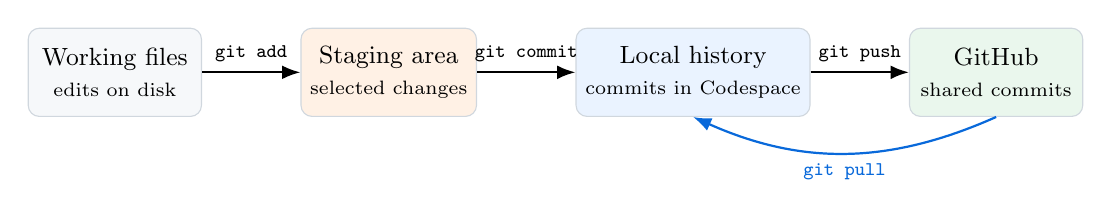
\begin{tikzpicture}[
  >=Latex,node distance=1.25cm,
  box/.style={draw=Rule,rounded corners,minimum width=2.20cm,minimum height=1.12cm,align=center,font=\small}
]
  \node[box,fill=CodeBG] (work) {Working files\\\scriptsize edits on disk};
  \node[box,fill=LightOrange,right=of work] (stage) {Staging area\\\scriptsize selected changes};
  \node[box,fill=LightBlue,right=of stage] (local) {Local history\\\scriptsize commits in Codespace};
  \node[box,fill=LightGreen,right=of local] (remote) {GitHub\\\scriptsize shared commits};
  \draw[->,thick] (work) -- node[above,font=\ttfamily\scriptsize]{git add} (stage);
  \draw[->,thick] (stage) -- node[above,font=\ttfamily\scriptsize]{git commit} (local);
  \draw[->,thick] (local) -- node[above,font=\ttfamily\scriptsize]{git push} (remote);
  \draw[->,thick,Blue,bend left=24] (remote.south) to node[below,font=\ttfamily\scriptsize]{git pull} (local.south);
\end{tikzpicture}
\end{center}

\vspace{0.75em}
\begin{alertblock}{The distinction that prevents most confusion}
Saving a file, committing it, and pushing it are three separate actions.
\end{alertblock}
\end{frame}

% -----------------------------------------------------------------------------
\begin{frame}{Step 1: open GitHub's repository form}
\begin{columns}[T,onlytextwidth]
  \column{0.50\textwidth}
  \textbf{In the GitHub website}
  \begin{enumerate}
    \item Sign in at \texttt{github.com}.
    \item In the upper-right corner, click \button{+}.
    \item Select \button{New repository}.
  \end{enumerate}

  \column{0.46\textwidth}
  \begin{beamercolorbox}[rounded=true,sep=0.55em]{block body}
    \textbf{GitHub}\hfill \button{+}\quad\button{Profile}\\[0.5em]
    \hrule
    \vspace{0.5em}
    \hfill\begin{minipage}{0.62\linewidth}
      New repository\\
      Import repository\\
      New codespace\\
      New gist
    \end{minipage}
  \end{beamercolorbox}
\end{columns}

\vspace{0.8em}
\takeaway{A repository is the project folder plus the Git history attached to it.}
\end{frame}

% -----------------------------------------------------------------------------
\begin{frame}{Step 2: configure and create the repository}
\begin{columns}[T,onlytextwidth]
  \column{0.56\textwidth}
  \begin{beamercolorbox}[rounded=true,sep=0.65em]{block body}
    \textbf{Create a new repository}\\[0.45em]
    Owner \hfill \button{your-username}\\[0.3em]
    Repository name \hfill \button{growth-calculator}\\[0.3em]
    Description \hfill \texttt{A simple Python growth calculator}\\[0.3em]
    Visibility \hfill \(circ\) Public \quad \(\bullet\) Private\\[0.3em]
    Add a README file \hfill \(\checkmark\)\\[0.55em]
    \hfill\button{Create repository}
  \end{beamercolorbox}

  \column{0.40\textwidth}
  \textbf{Why add a README?}
  \begin{itemize}
    \item It explains the project to a visitor.
    \item It gives the repository a first file.
    \item GitHub creates the first commit for us.
  \end{itemize}
\end{columns}

\vspace{0.45em}
\statebadge{LightGreen}{Checkpoint: the repository exists on GitHub}
\end{frame}

% -----------------------------------------------------------------------------
\begin{frame}{Step 3: start a Codespace}
\begin{columns}[T,onlytextwidth]
  \column{0.48\textwidth}
  \textbf{From the repository page}
  \begin{enumerate}
    \item Click the green \button{Code} button.
    \item Select the \button{Codespaces} tab.
    \item Click \button{Create codespace on main}.
  \end{enumerate}
  GitHub opens a new browser tab. Starting the cloud computer can take a minute.

  \column{0.48\textwidth}
  \begin{beamercolorbox}[rounded=true,sep=0.65em]{block body example}
    \textbf{growth-calculator}\hfill\button{Code}\\[0.6em]
    \button{Local}\quad\button{Codespaces}\\[0.7em]
    \centering\button{Create codespace on main}
  \end{beamercolorbox}
\end{columns}

\vspace{0.7em}
\takeaway{The Codespace contains a working copy of the GitHub repository.}
\end{frame}

% -----------------------------------------------------------------------------
\begin{frame}{Orient yourself inside Codespaces}
\begin{columns}[T,onlytextwidth]
  \column{0.62\textwidth}
  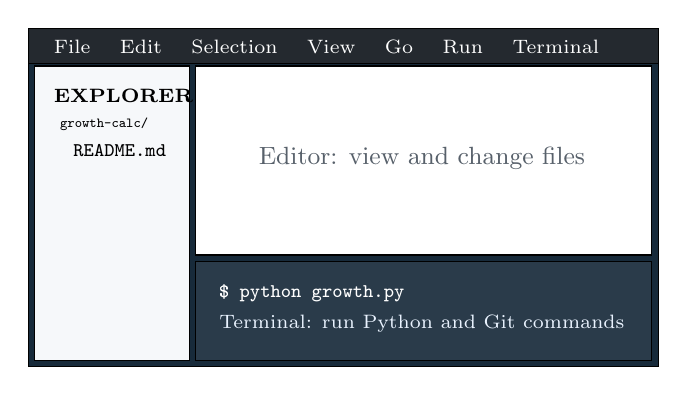
\begin{tikzpicture}[x=1cm,y=1cm]
    \draw[fill=Navy] (0,0) rectangle (8.0,4.3);
    \draw[fill=Ink] (0,3.85) rectangle (8.0,4.3);
    \node[anchor=west,text=white,font=\scriptsize] at (0.2,4.07) {File \quad Edit \quad Selection \quad View \quad Go \quad Run \quad Terminal};
    \draw[fill=CodeBG] (0.08,0.08) rectangle (2.05,3.82);
    \node[anchor=north west,font=\bfseries\scriptsize] at (0.2,3.65) {EXPLORER};
    \node[anchor=north west,font=\ttfamily\tiny] at (0.28,3.28) {growth-calc/};
    \node[anchor=north west,font=\ttfamily\scriptsize] at (0.45,2.95) {README.md};
    \draw[fill=white] (2.12,1.42) rectangle (7.92,3.82);
    \node[text=Muted,font=\small] at (5.0,2.65) {Editor: view and change files};
    \draw[fill=Navy!92] (2.12,0.08) rectangle (7.92,1.34);
    \node[anchor=north west,text=white,font=\ttfamily\scriptsize] at (2.3,1.17) {\$ python growth.py};
    \node[text=LightBlue,font=\scriptsize] at (5.0,0.55) {Terminal: run Python and Git commands};
  \end{tikzpicture}

  \column{0.34\textwidth}
  \textbf{The areas we will use}
  \begin{itemize}
    \item \textbf{Explorer:} create and open files.
    \item \textbf{Editor:} write code.
    \item \textbf{Terminal:} run commands.
  \end{itemize}
  Open the terminal with:
  \begin{center}
    \button{Terminal} \(\rightarrow\) \button{New Terminal}
  \end{center}
\end{columns}
\end{frame}

% -----------------------------------------------------------------------------
\begin{frame}[fragile]{Inspect the starting repository}
\begin{columns}[T,onlytextwidth]
  \column{0.54\textwidth}
  \textbf{Type in the terminal}
\begin{lstlisting}[style=terminal]
$ pwd
/workspaces/growth-calculator
$ ls
README.md
$ git status
On branch main
Your branch is up to date with 'origin/main'.
nothing to commit, working tree clean
\end{lstlisting}

  \column{0.42\textwidth}
  \textbf{How to read this}
  \begin{itemize}
    \item \texttt{pwd}: show the current folder.
    \item \texttt{ls}: list the files in it.
    \item \texttt{main}: the current branch.
    \item \texttt{origin/main}: GitHub's corresponding branch.
    \item \texttt{clean}: no unsaved Git changes.
  \end{itemize}
\end{columns}

\vspace{0.65em}\begin{center}\statebadge{LightGreen}{Checkpoint: both copies are synchronized}\end{center}
\end{frame}

% -----------------------------------------------------------------------------
\begin{frame}[fragile]{Read the existing history}
\begin{columns}[T,onlytextwidth]
  \column{0.48\textwidth}
  \textbf{Type}
\begin{lstlisting}[style=terminal]
$ git log --oneline
a1b2c3d (HEAD -> main, origin/main)
        Initial commit
\end{lstlisting}

  \column{0.48\textwidth}
  \textbf{Interpret the output}
  \begin{itemize}
    \item \texttt{a1b2c3d}: shortened commit identifier.
    \item \texttt{HEAD -> main}: where our Codespace currently points.
    \item \texttt{origin/main}: where GitHub currently points.
    \item \texttt{Initial commit}: the saved description.
  \end{itemize}
\end{columns}

\vspace{0.8em}
\takeaway{Both labels point to the same commit, so the two copies are synchronized.}
\end{frame}

% -----------------------------------------------------------------------------
\begin{frame}[fragile]{Create the program: \texttt{growth.py}}
\begin{columns}[T,onlytextwidth]
  \column{0.38\textwidth}
  \textbf{In the Explorer}
  \begin{enumerate}
    \item Click the \button{New File} icon.
    \item Name the file \texttt{growth.py}.
    \item Enter the code shown here.
    \item Save with \button{Ctrl+S}.
  \end{enumerate}
  No package installation is needed.

  \column{0.58\textwidth}
\begin{lstlisting}[style=code,language=Python]
def percentage_change(old_value, new_value):
    """Return percentage change from old to new."""
    if old_value == 0:
        raise ValueError("old_value cannot be zero")

    return 100 * (new_value - old_value) / old_value


if __name__ == "__main__":
    result = percentage_change(100, 105)
    print(f"Percentage change: {result}%")
\end{lstlisting}
\end{columns}
\end{frame}

% -----------------------------------------------------------------------------
\begin{frame}[fragile]{Run the program before saving a Git version}
\begin{columns}[T,onlytextwidth]
  \column{0.54\textwidth}
  \textbf{Type}
\begin{lstlisting}[style=terminal]
$ python growth.py
Percentage change: 5.0%
\end{lstlisting}

  Try a different pair of values by changing:
\begin{lstlisting}[style=code,language=Python]
result = percentage_change(100, 105)
\end{lstlisting}

  \column{0.42\textwidth}
  \textbf{What just happened?}
  \begin{itemize}
    \item Python executed the file.
    \item The program produced the expected result.
    \item Git has not saved a new version.
    \item GitHub has not received anything.
  \end{itemize}
\end{columns}

\vspace{0.55em}
\takeaway{Running code and recording its version are separate actions.}
\end{frame}

% -----------------------------------------------------------------------------
\begin{frame}[fragile]{Ask Git what changed}
\begin{columns}[T,onlytextwidth]
  \column{0.54\textwidth}
\begin{lstlisting}[style=terminal]
$ git status
On branch main
Untracked files:
  (use "git add <file>..." to include in what
   will be committed)
        growth.py

nothing added to commit
\end{lstlisting}

  \column{0.42\textwidth}
  \textbf{``Untracked'' means}
  \begin{itemize}
    \item the file exists in the Codespace;
    \item Git sees it;
    \item it has never been included in a commit.
  \end{itemize}
  \begin{alertblock}{A useful subtlety}
    \texttt{git diff} shows changes to tracked files. It will not display the contents of this new, untracked file.
  \end{alertblock}
\end{columns}
\end{frame}

% -----------------------------------------------------------------------------
\begin{frame}[fragile]{Stage the file, then review exactly what is staged}
\begin{columns}[T,onlytextwidth]
  \column{0.54\textwidth}
\begin{lstlisting}[style=terminal]
$ git add growth.py
$ git status
Changes to be committed:
        new file:   growth.py

$ git diff --staged
diff --git a/growth.py b/growth.py
new file mode 100644
--- /dev/null
+++ b/growth.py
@@ ...
+def percentage_change(old_value, new_value):
\end{lstlisting}

  \column{0.42\textwidth}
  \textbf{What changed in Git?}
  \begin{itemize}
    \item \texttt{git add} selected \texttt{growth.py} for the next commit.
    \item It did not create the commit.
    \item \texttt{git diff --staged} previews the exact snapshot.
  \end{itemize}
  \statebadge{LightOrange}{State: staged, not committed}
\end{columns}
\end{frame}

% -----------------------------------------------------------------------------
\begin{frame}[fragile]{Commit: save one coherent change}
\begin{columns}[T,onlytextwidth]
  \column{0.54\textwidth}
\begin{lstlisting}[style=terminal]
$ git commit -m "Add growth calculator"
[main d4e5f6a] Add growth calculator
 1 file changed, 11 insertions(+)
 create mode 100644 growth.py

$ git log --oneline
d4e5f6a (HEAD -> main) Add growth calculator
a1b2c3d (origin/main) Initial commit
\end{lstlisting}

  \column{0.42\textwidth}
  \textbf{How to read this}
  \begin{itemize}
    \item The commit identifier is \texttt{d4e5f6a}.
    \item \texttt{HEAD -> main} moved to the new commit.
    \item \texttt{origin/main} did not move.
    \item The commit exists locally, not yet on GitHub.
  \end{itemize}
  \statebadge{LightBlue}{State: committed locally}
\end{columns}
\end{frame}

% -----------------------------------------------------------------------------
\begin{frame}[fragile]{Push: send local commits to GitHub}
\begin{columns}[T,onlytextwidth]
  \column{0.52\textwidth}
\begin{lstlisting}[style=terminal]
$ git push
Enumerating objects: 4, done.
Writing objects: 100% (3/3), done.
To https://github.com/your-username/
growth-calculator.git
   a1b2c3d..d4e5f6a  main -> main
\end{lstlisting}
  Then return to the GitHub tab and refresh the repository page.

  \column{0.44\textwidth}
  \textbf{Verify on GitHub}
  \begin{enumerate}
    \item Is \texttt{growth.py} visible?
    \item Is the commit message visible?
    \item Does the commit history show two commits?
  \end{enumerate}
  \begin{exampleblock}{Why verification matters}
    A successful local commit does not imply a successful push.
  \end{exampleblock}
\end{columns}

\statebadge{LightGreen}{Checkpoint: Codespace and GitHub contain the new commit}
\end{frame}

% -----------------------------------------------------------------------------
\begin{frame}[fragile]{Create package-free tests: \texttt{test\_growth.py}}
\begin{columns}[T,onlytextwidth]
  \column{0.38\textwidth}
  Create a new file named \texttt{test\_growth.py}.

  Each \texttt{assert} states a result that must be true. If one is false, Python stops with an error.

  \begin{block}{No installed packages}
    \texttt{growth} refers to our own \texttt{growth.py} file. The tests use only Python itself.
  \end{block}

  \column{0.58\textwidth}
\begin{lstlisting}[style=code,language=Python]
from growth import percentage_change


assert percentage_change(100, 105) == 5
assert percentage_change(100, 90) == -10
assert percentage_change(100, 100) == 0

print("All tests passed.")
\end{lstlisting}
\end{columns}
\end{frame}

% -----------------------------------------------------------------------------
\begin{frame}[fragile]{Run the tests---and see what failure looks like}
\begin{columns}[T,onlytextwidth]
  \column{0.49\textwidth}
  \textbf{When all expectations are correct}
\begin{lstlisting}[style=terminal]
$ python test_growth.py
All tests passed.
\end{lstlisting}

  Temporarily change the first expected result from \texttt{5} to \texttt{6} and rerun.

  \column{0.47\textwidth}
  \textbf{A failing test}
\begin{lstlisting}[style=terminal]
$ python test_growth.py
Traceback (most recent call last):
  File "test_growth.py", line 4
    assert percentage_change(100,105) == 6
AssertionError
\end{lstlisting}
  Restore \texttt{5} and rerun until all tests pass.
\end{columns}

\vspace{0.45em}
\takeaway{A test converts an expected result into a check the computer can repeat.}
\end{frame}

% -----------------------------------------------------------------------------
\begin{frame}[fragile]{Record the tested change}
\begin{columns}[T,onlytextwidth]
  \column{0.55\textwidth}
\begin{lstlisting}[style=terminal]
$ git status
$ git diff
$ python test_growth.py
All tests passed.
$ git add test_growth.py
$ git diff --staged
$ git commit -m "Add tests for growth calculator"
$ git push
\end{lstlisting}

  \column{0.41\textwidth}
  \textbf{Why this order?}
  \begin{enumerate}
    \item Identify changed files.
    \item Inspect their contents.
    \item Verify the code works.
    \item Select the intended change.
    \item Review, commit, and share it.
  \end{enumerate}
\end{columns}

\vspace{0.45em}
\takeaway{A good commit is small, coherent, reviewed, and tested.}
\end{frame}

% -----------------------------------------------------------------------------
\begin{frame}{Simulate a collaborator by editing on GitHub}
\begin{columns}[T,onlytextwidth]
  \column{0.52\textwidth}
  \textbf{On the GitHub repository page}
  \begin{enumerate}
    \item Click \texttt{README.md}.
    \item Click the pencil icon \button{Edit this file}.
    \item Add the text shown at right.
    \item Click \button{Commit changes...}.
    \item Enter \texttt{Describe the project} and confirm.
  \end{enumerate}

  \column{0.44\textwidth}
  \begin{beamercolorbox}[rounded=true,sep=0.65em]{block body}
    \textbf{README.md}\hfill\button{Edit}\\[0.5em]
    \ttfamily\small
    \# Growth calculator\\[0.25em]
    A small Python program that calculates percentage changes.
  \end{beamercolorbox}
\end{columns}

\vspace{0.65em}
\statebadge{LightOrange}{Now GitHub is one commit ahead of the Codespace}
\end{frame}

% -----------------------------------------------------------------------------
\begin{frame}[fragile]{Fetch, inspect, then pull the new commit}
\begin{columns}[T,onlytextwidth]
  \column{0.59\textwidth}
\begin{lstlisting}[style=terminal]
$ git fetch
From https://github.com/.../growth-calculator
   6141a87..5f89e4d  main -> origin/main

$ git status
On branch main
Your branch is behind 'origin/main' by 1 commit,
and can be fast-forwarded.
  (use "git pull" to update your local branch)

$ git pull
Updating 6141a87..5f89e4d
Fast-forward
 README.md | 3 +++
 1 file changed, 3 insertions(+)
\end{lstlisting}

  \column{0.37\textwidth}
  \textbf{What each command does}
  \begin{enumerate}
    \item \texttt{git fetch} contacts GitHub and refreshes \texttt{origin/main}; it does not change your files.
    \item \texttt{git status} now sees that GitHub is one commit ahead.
    \item \texttt{git pull} moves \texttt{main} forward and updates \texttt{README.md}.
  \end{enumerate}
  ``Fast-forward'' means there was no competing local commit to merge.
\end{columns}


\end{frame}

% -----------------------------------------------------------------------------
\begin{frame}{What is \texttt{.gitignore}?}
\begin{columns}[T,onlytextwidth]
  \column{0.48\textwidth}
  \begin{block}{A plain-text instruction file}
    We create \texttt{.gitignore} to tell Git which files or folders it should not track.
  \end{block}
  Each line names a path or pattern to ignore. That line is sometimes called a ``rule.''

  \column{0.48\textwidth}
  For this project, the complete file is:
\begin{beamercolorbox}[rounded=true,sep=0.8em]{block body}
\ttfamily\large
\_\_pycache\_\_/
\end{beamercolorbox}
  \vspace{0.55em}
  This one line means: ``Git, ignore the \texttt{\_\_pycache\_\_/} directory that Python created.''
\end{columns}

\vspace{0.55em}
\begin{alertblock}{Nothing is deleted}
The directory stays on the computer. Git simply stops offering to include it in commits.
\end{alertblock}
\end{frame}

% -----------------------------------------------------------------------------
\begin{frame}[fragile]{Create, check, and commit \texttt{.gitignore}}
\begin{columns}[T,onlytextwidth]
  \column{0.51\textwidth}
  \textbf{1. Create the file}
\begin{lstlisting}[style=terminal]
$ printf "__pycache__/\n" > .gitignore
$ cat .gitignore
__pycache__/
\end{lstlisting}
  \texttt{printf} writes the line into \texttt{.gitignore}; \texttt{cat} checks what was written.

  \textbf{2. Check the result}
\begin{lstlisting}[style=terminal]
$ git status --short
?? .gitignore
\end{lstlisting}
  The cache is no longer listed because Git is ignoring it.

  \column{0.45\textwidth}
  \textbf{3. Share the instruction}
\begin{lstlisting}[style=terminal]
$ git add .gitignore
$ git commit -m "Ignore Python cache"
$ git push
\end{lstlisting}
  We commit \texttt{.gitignore} so everyone using the repository gets the same instruction.

  \vspace{0.55em}
  \begin{beamercolorbox}[rounded=true,sep=0.65em]{block body example}
    \textbf{Tracked:} \texttt{.gitignore}\\
    \textbf{Ignored:} \texttt{\_\_pycache\_\_/}
  \end{beamercolorbox}
\end{columns}
\end{frame}

% -----------------------------------------------------------------------------
\begin{frame}[fragile]{If a push is rejected, synchronize first}
\begin{columns}[T,onlytextwidth]
  \column{0.52\textwidth}
\begin{lstlisting}[style=terminal]
$ git push
! [rejected] main -> main (fetch first)
error: failed to push some refs
\end{lstlisting}
  This means GitHub has commits that your Codespace does not have. Git refuses to overwrite them.

  \column{0.44\textwidth}
  \textbf{Safe response}
\begin{lstlisting}[style=terminal]
$ git status
$ git pull
# Read any message from Git carefully.
$ python test_growth.py
$ git push
\end{lstlisting}
  If Git reports a conflict, stop and resolve the marked files before pushing.
\end{columns}

\vspace{0.4em}
\begin{alertblock}{Do not solve this with force}
For this course workflow, do not use \texttt{git push --force}: it can discard shared history.
\end{alertblock}
\end{frame}

% -----------------------------------------------------------------------------
\begin{frame}{What is a merge conflict?}
\begin{columns}[T,onlytextwidth]
  \column{0.50\textwidth}
  A conflict occurs when Git cannot decide how to combine competing edits automatically.

  Git marks the disputed region:
  \begin{beamercolorbox}[rounded=true,sep=0.55em]{block body alerted}
    \ttfamily\scriptsize
    <<<<<<< HEAD\\
    Percentage change calculator\\
    =======\\
    Growth rate calculator\\
    >>>>>>> origin/main
  \end{beamercolorbox}

  \column{0.46\textwidth}
  \textbf{Resolution procedure}
  \begin{enumerate}
    \item Read both versions.
    \item Edit the file to the intended final content.
    \item Remove all conflict markers.
    \item Run the program and tests.
    \item Stage and commit the resolution.
  \end{enumerate}
\end{columns}

\vspace{0.4em}
\takeaway{A conflict is a request for human judgment, not evidence that work was lost.}
\end{frame}

% -----------------------------------------------------------------------------
\begin{frame}{The daily workflow}
\begin{center}
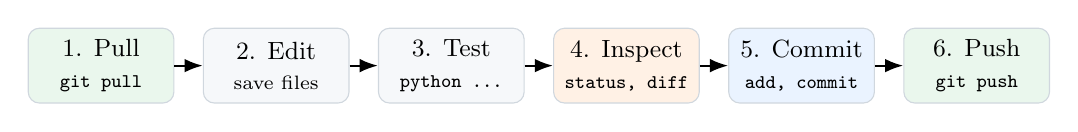
\begin{tikzpicture}[
  >=Latex,node distance=0.36cm,
  every node/.style={font=\small},
  stagebox/.style={draw=Rule,rounded corners,minimum width=1.85cm,minimum height=0.95cm,align=center}
]
  \node[stagebox,fill=LightGreen] (pull) {1. Pull\\\ttfamily\scriptsize git pull};
  \node[stagebox,fill=CodeBG,right=of pull] (edit) {2. Edit\\\scriptsize save files};
  \node[stagebox,fill=CodeBG,right=of edit] (test) {3. Test\\\ttfamily\scriptsize python ...};
  \node[stagebox,fill=LightOrange,right=of test] (inspect) {4. Inspect\\\ttfamily\scriptsize status, diff};
  \node[stagebox,fill=LightBlue,right=of inspect] (commit) {5. Commit\\\ttfamily\scriptsize add, commit};
  \node[stagebox,fill=LightGreen,right=of commit] (push) {6. Push\\\ttfamily\scriptsize git push};
  \foreach \a/\b in {pull/edit,edit/test,test/inspect,inspect/commit,commit/push}
    \draw[->,thick] (\a) -- (\b);
\end{tikzpicture}
\end{center}

\vspace{0.7em}
\begin{columns}[T,onlytextwidth]
  \column{0.48\textwidth}
  \textbf{Before the commit}
  \begin{itemize}
    \item Does the program run?
    \item Do the tests pass?
    \item Did I inspect every changed line?
  \end{itemize}
  \column{0.48\textwidth}
  \textbf{After the commit}
  \begin{itemize}
    \item Is the message meaningful?
    \item Did the push succeed?
    \item Can I see the commit on GitHub?
  \end{itemize}
\end{columns}
\end{frame}

% -----------------------------------------------------------------------------
\begin{frame}[fragile]{Your turn: make one complete change}
\begin{columns}[T,onlytextwidth]
  \column{0.48\textwidth}
  \textbf{Choose one improvement}
  \begin{itemize}
    \item Add a test using values \texttt{200} and \texttt{210}.
    \item Change the displayed example.
    \item Improve the function's docstring.
    \item Add instructions to \texttt{README.md}.
  \end{itemize}

  \column{0.48\textwidth}
  \textbf{Complete the whole cycle}
\begin{lstlisting}[style=terminal]
$ git pull
# Edit and save the chosen file.
$ python growth.py
$ python test_growth.py
$ git status
$ git diff
$ git add <the-file-you-changed>
$ git diff --staged
$ git commit -m "Describe the improvement"
$ git push
\end{lstlisting}
\end{columns}

\vspace{0.3em}
\statebadge{LightGreen}{Done means: the new commit is visible on GitHub}
\end{frame}

% -----------------------------------------------------------------------------
\begin{frame}[fragile]{Command guide: question first, command second}
\small
\begin{tabular}{@{}p{0.46\textwidth}p{0.43\textwidth}@{}}
\toprule
\textbf{Question} & \textbf{Command} \\
\midrule
What is the repository's current state? & \texttt{git status} \\
What unstaged tracked lines changed? & \texttt{git diff} \\
What exactly is selected for the next commit? & \texttt{git diff --staged} \\
Which changes should enter the next commit? & \texttt{git add <file>} \\
How do I save the staged snapshot? & \texttt{git commit -m "message"} \\
What commits exist in the history? & \texttt{git log --oneline} \\
How do I receive GitHub's newer commits? & \texttt{git pull} \\
How do I send my local commits to GitHub? & \texttt{git push} \\
\bottomrule
\end{tabular}

\vspace{0.7em}
\takeaway{When uncertain, start with \texttt{git status}; read Git's message before acting.}
\end{frame}

% -----------------------------------------------------------------------------
\begin{frame}{The one picture to remember}
\begin{center}
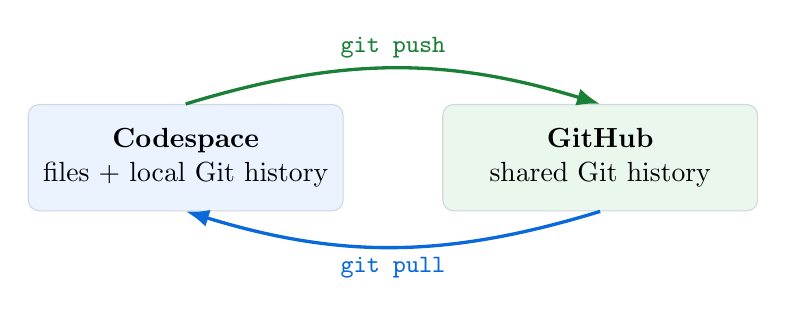
\begin{tikzpicture}[
  >=Latex,node distance=1.25cm,
  box/.style={draw=Rule,rounded corners,minimum width=4.0cm,minimum height=1.35cm,align=center}
]
  \node[box,fill=LightBlue] (code) {\textbf{Codespace}\\files + local Git history};
  \node[box,fill=LightGreen,right=of code] (hub) {\textbf{GitHub}\\shared Git history};
  \draw[->,very thick,Green,bend left=17] (code.north) to node[above,font=\ttfamily\small]{git push} (hub.north);
  \draw[->,very thick,Blue,bend left=17] (hub.south) to node[below,font=\ttfamily\small]{git pull} (code.south);
\end{tikzpicture}
\end{center}

\vspace{0.6em}
\begin{center}
  \Large\bfseries
  Pull \(\rightarrow\) Edit \(\rightarrow\) Test \(\rightarrow\) Inspect
  \(\rightarrow\) Commit \(\rightarrow\) Push
\end{center}

\vspace{0.5em}
\begin{center}
  \color{Muted}Use it on every project until the workflow becomes routine.
\end{center}
\end{frame}

\end{document}
